\documentclass[a4paper,11.5pt,table]{article}
\usepackage[textwidth=170mm, textheight=230mm, inner=20mm, top=20mm, bottom=30mm]{geometry}
\usepackage[normalem]{ulem}
\usepackage[utf8]{inputenc}
\usepackage[T1]{fontenc}
\PassOptionsToPackage{defaults=hu-min}{magyar.ldf}
\usepackage[magyar]{babel}
\usepackage{amsmath, amsthm,amssymb, paralist, tikz, multirow}
\usetikzlibrary{shapes.geometric, arrows, positioning, math, calc}
\begin{document}
%	\begin{figure}[!h]
%		\centering
%		\begin{tikzpicture}[
%				triangle/.style = {
%					shape=isosceles triangle,
%					shape border rotate = 90
%				},
%				level 1/.style={level distance=1cm},
%				level 2/.style={sibling distance=3cm},
%				level 3/.style={sibling distance=1.5cm},
%				edge from parent/.style={draw=none}
%			]
%			\tikzstyle{Node} = [ %describes the basic look of the shapes
%				text centered, 
%				draw=black, 
%				fill= gray!20
%			]
%			\tikzstyle{CircNode} = [
%				circle,
%				minimum width=6mm,
%				Node
%			]
%			\tikzstyle{TriNode} = [
%				triangle,
%				minimum width=13mm, 
%				minimum height=13mm,
%				isosceles triangle stretches,
%				Node
%			]
%			
%			\node (t1) {$t$}
%			child {
%				node (T1) [CircNode]{T}
%				child [level distance=20mm]{
%					node (a1) [TriNode]{$\alpha$}
%				}
%				child [level distance=13mm]{
%					node (R1) [CircNode]{R}
%					child {
%						node (b1) [TriNode]{$\beta$}
%					}
%					child [level distance = 18mm] {
%						node (c1) [TriNode, minimum height=18mm]{$\gamma$}
%					}
%				}
%			};
%			\draw[->, thick] (t1) -- (T1);
%			\draw[->, thick] (T1) -- (R1);
%			\draw[->, thick] (T1) -- (-1.5,-2.05);
%			\draw[->, thick] (R1) -- (0.75,-2.65);
%			\draw[->, thick] (R1) -- (2.25,-2.7);
%			\node [right = 0mm of T1] {\texttt{++}};
%			\node [right = 0mm of R1] {\texttt{+}};
%			\node [below = 0mm of a1] {$h$};
%			\node [below = 0mm of b1] {$h$};
%			\node [below = 0mm of c1] {$h+1$};
%			\draw[<->, thick] (-2.5, -4.5) -- node [anchor=center, left, text width= 1.5cm, text centered]{$h(t)=$\\$h+3$}(-2.5, 0.1);
%			
%			\draw[->, thick] (3.2,-2) -- (4.2,-2) node [midway, above] {L};
%			
%			\node (t2)[right = 7 cm of t1] {$t$}
%			child {
%				node (R2) [CircNode]{R}
%				child{
%					node (T2) [CircNode] {T}
%					[level distance = 15mm]
%					child {
%						node (a2) [TriNode]{$\alpha$}
%					}
%					child{
%						node (b2)[TriNode]{$\beta$}
%					}
%				}
%				child[level distance = 24.5mm] {
%					node (c2) [TriNode, minimum height=18mm] {$\gamma$}
%				}
%			};
%			\draw[->, thick] (t2) -- (R2);
%			\draw[->, thick] (R2) -- (T2);
%			\draw[->, thick] (T2) -- (5.1,-2.6);
%			\draw[->, thick] (T2) -- (6.65,-2.6);
%			\draw[->, thick] (R2) -- (8.9,-2.1);
%			\node [right = 0mm of T2] {\texttt{0}};
%			\node [right = 0mm of R2] {\texttt{0}};
%			\node [below = 0mm of a2] {$h$};
%			\node [below = 0mm of b2] {$h$};
%			\node [below = 0mm of c2] {$h+1$};
%			\draw[<->, thick] (10, -3.9) -- node [anchor=center, right, text width= 1.5cm, text centered]{$h(t)=$\\$h+2$}(10, 0.1);
%		\end{tikzpicture}
%		\caption{Jegyezzük meg, hogy a $h(t)$ szimbólum a $t$ fa, míg a $h$ szimbólum az $\alpha$ és $\beta$ részfák magasságát jelenti.}
%	\end{figure}
%
%	\begin{figure}[!h]
%		\centering
%		\begin{tikzpicture}[
%				triangle/.style = {
%					shape=isosceles triangle,
%					shape border rotate = 90
%				},
%				level 1/.style={level distance=1cm},
%				level 2/.style={sibling distance=3cm},
%				level 3/.style={sibling distance=1.5cm},
%				edge from parent/.style={draw=none}
%			]
%			\tikzstyle{Node} = [ %describes the basic look of the shapes
%				text centered, 
%				draw=black, 
%				fill= gray!20
%			]
%			\tikzstyle{CircNode} = [
%				circle,
%				minimum width=6mm,
%				Node
%			]
%			\tikzstyle{TriNode} = [
%				triangle,
%				minimum width=13mm, 
%				minimum height=13mm,
%				isosceles triangle stretches,
%				Node
%			]
%			
%			\node (t1) {$t$}
%			child {
%				node (T1) [CircNode]{T}
%				child [level distance=13mm]{
%					node (R1) [CircNode]{R}
%					child [level distance = 18mm] {
%						node (a1) [TriNode, minimum height=18mm]{$\alpha$}
%					}
%					child {
%						node (b1) [TriNode]{$\beta$}
%					}
%				}
%				child [level distance=20mm]{
%					node (c1) [TriNode]{$\gamma$}
%				}
%			};
%			\draw[->, thick] (t1) -- (T1);
%			\draw[->, thick] (T1) -- (R1);
%			\draw[->, thick] (T1) -- (1.5,-2.05);
%			\draw[->, thick] (R1) -- (-0.75,-2.65);
%			\draw[->, thick] (R1) -- (-2.25,-2.7);
%			\node [right = 0mm of T1] {\texttt{-\hspace{0mm}-}};
%			\node [right = 0mm of R1] {\texttt{-}};
%			\node [below = 0mm of a1] {$h+1$};
%			\node [below = 0mm of c1] {$h$};
%			\node [below = 0mm of b1] {$h$};
%			\draw[<->, thick] (-3.2, -4.5) -- node [anchor=center, left, text width= 1.5cm, text centered]{$h(t)=$\\$h+3$}(-3.2, 0.1);
%			
%			\draw[->, thick] (2.7,-2) -- (3.7,-2) node [midway, above] {R};
%			
%			\node (t2)[right = 6 cm of t1] {$t$}
%			child {
%				node (R2) [CircNode]{R}
%				child[level distance = 24.5mm] {
%					node (a2) [TriNode, minimum height=18mm]{$\alpha$}
%				}
%				child{
%					node (T2) [CircNode] {T}
%					[level distance = 15mm]
%					child {
%						node (b2)[TriNode]{$\beta$}
%					}
%					child{
%						node (c2) [TriNode]{$\gamma$}
%					}
%				}
%			};
%			\draw[->, thick] (t2) -- (R2);
%			\draw[->, thick] (R2) -- (T2);
%			\draw[->, thick] (T2) -- (7.1,-2.6);
%			\draw[->, thick] (T2) -- (8.65,-2.6);
%			\draw[->, thick] (R2) -- (4.85,-2.07);
%			\node [right = 0mm of T2] {\texttt{0}};
%			\node [right = 0mm of R2] {\texttt{0}};
%			\node [below = 0mm of a2] {$h+1$};
%			\node [below = 0mm of c2] {$h$};
%			\node [below = 0mm of b2] {$h$};
%			\draw[<->, thick] (9.7, -3.9) -- node [anchor=center, right, text width= 1.5cm, text centered]{$h(t)=$\\$h+2$}(9.7, 0.1);
%		\end{tikzpicture}
%		\caption{Jegyezzük meg, hogy a $h(t)$ szimbólum a $t$ fa, míg a $h$ szimbólum az $\alpha$ és $\beta$ részfák magasságát jelenti.}
%	\end{figure}	
%
%	\begin{figure}[!h]
%		\centering
%		\begin{tikzpicture}[
%				triangle/.style = {
%					shape=isosceles triangle,
%					shape border rotate = 90
%				},
%				level 1/.style={level distance=1cm},
%				level 2/.style={sibling distance=3cm},
%				level 3/.style={sibling distance=1.5cm},
%				edge from parent/.style={draw=none}
%			]
%			\tikzstyle{Node} = [ %describes the basic look of the shapes
%				text centered, 
%				draw=black, 
%				fill= gray!20
%			]
%			\tikzstyle{CircNode} = [
%				circle,
%				minimum width=6mm,
%				Node
%			]
%			\tikzstyle{TriNode} = [
%				triangle,
%				minimum width=13mm, 
%				minimum height=13mm,
%				isosceles triangle stretches,
%				Node
%			]
%			
%			\node (t1) {$t$}
%			child {
%				node (T1) [CircNode]{T}
%				child [level distance=31mm]{
%					node (a1) [TriNode]{$\alpha$}
%				}
%				child [level distance=10mm]{
%					node (R1) [CircNode]{R}
%					child [level distance = 10mm] {
%						node (L1) [CircNode]{L}
%						child [level distance = 15mm] {
%							node (b1) [TriNode]{$\beta$}
%						}
%						child [level distance = 15mm]{
%							node (c1) [TriNode]{$\gamma$}
%						}
%					}
%					child [level distance = 20mm, sibling distance = 25mm] {
%						node (d1) [TriNode]{$\delta$}
%					}
%				}
%			};
%			\draw[->, thick] (t1) -- (T1);
%			\draw[->, thick] (T1) -- (R1);
%			\draw[->, thick] (R1) -- (L1);
%			\draw[->, thick] (T1) -- (-1.5,-3.15);
%			\draw[->, thick] (R1) -- (2.75,-3.1);
%			\draw[->, thick] (L1) -- (0,-3.55);
%			\draw[->, thick] (L1) -- (1.5,-3.55);
%			\node [right = 0mm of T1] {\texttt{++}};
%			\node [right = 0mm of R1] {\texttt{-}};
%			\node [right = 0mm of L1, text width= 1.5cm] {\texttt{-}\\ \vspace{-1.5mm}\texttt{0}\\ \vspace{-1.5mm}\texttt{+}};
%			\node [below = 0mm of a1] {$h$};
%			\node [below = 0mm of b1, text width= 1cm, text centered] {$h$\\$h$\\$h-1$};
%			\node [below = 0mm of c1, text width= 1cm, text centered] {$h-1$\\$h$\\$h$};
%			\node [below = 0mm of d1] {$h$};
%%			\draw[<->, thick] (-2.7, -4.85) -- node [anchor=center, left, text width= 1.5cm, text centered]{$h(t)=$\\$h+4$}(-2.7, 0.1);
%			
%			\draw[->, thick] (3.6,-2) -- (4.6,-2) node [midway, above] {RL};
%			
%			\node (t2) [right = 7.5cm of t1] {$t$}
%			child {
%				node (R2) [CircNode]{R}
%				child [level distance = 10mm] {
%					[level distance=15mm]
%					node (L2) [CircNode]{L}
%					child{
%						node (a2) [TriNode]{$\alpha$}
%					}
%					child{
%						node (b2) [TriNode]{$\beta$}
%					}
%				}
%				child {
%					[level distance=15mm]
%					node (T2) [CircNode]{T}
%					child {
%						node (c2) [TriNode]{$\gamma$}
%					}
%					child{
%						node (d2) [TriNode]{$\delta$}
%					}
%				}
%			};
%			\draw[->, thick] (t2) -- (R2);
%			\draw[->, thick] (R2) -- (T2);
%			\draw[->, thick] (R2) -- (L2);
%			\draw[->, thick] (L2) -- (5.65,-2.55);
%			\draw[->, thick] (L2) -- (7.13,-2.55);
%			\draw[->, thick] (T2) -- (8.6,-2.55);
%			\draw[->, thick] (T2) -- (10.15,-2.55);
%			\node [right = 0mm of R2] {\texttt{0}};
%			\node [left = 1mm of L2, text width= 2mm] {\texttt{0}\\ \vspace{-1.5mm}\texttt{0}\\ \vspace{-1.5mm}\texttt{-}};
%			\node [right = 1mm of T2, text width= 1.5cm] {\texttt{+}\\ \vspace{-1.5mm}\texttt{0}\\ \vspace{-1.5mm}\texttt{0}};
%			\node [below = 0mm of a2] {$h$};
%			\node [below = 0mm of b2, text width= 1cm, text centered] {$h$\\$h$\\$h-1$};
%			\node [below = 0mm of c2, text width= 1cm, text centered] {$h-1$\\$h$\\$h$};
%			\node [below = 0mm of d2] {$h$};
%%			\draw[<->, thick] (11.2, -3.9) -- node [anchor=center, right, text width= 1.5cm, text centered]{$h(t)=$\\$h+2$}(11.2, 0.1);
%		\end{tikzpicture}
%		\caption{Jegyezzük meg, hogy a $h(t)$ szimbólum a $t$ fa, míg a $h$ szimbólum az $\alpha$ és $\beta$ részfák magasságát jelenti.}
%	\end{figure}	
%
%	\begin{figure}[!h]
%		\centering
%		\begin{tikzpicture}[
%				triangle/.style = {
%					shape=isosceles triangle,
%					shape border rotate = 90
%				},
%				level 1/.style={level distance=1cm},
%				level 2/.style={sibling distance=3cm},
%				level 3/.style={sibling distance=1.5cm},
%				edge from parent/.style={draw=none}
%			]
%			\tikzstyle{Node} = [ %describes the basic look of the shapes
%				text centered, 
%				draw=black, 
%				fill= gray!20
%			]
%			\tikzstyle{CircNode} = [
%				circle,
%				minimum width=6mm,
%				Node
%			]
%			\tikzstyle{TriNode} = [
%				triangle,
%				minimum width=13mm, 
%				minimum height=13mm,
%				isosceles triangle stretches,
%				Node
%			]
%			
%			\node (t1) {$t$}
%			child {
%				node (T1) [CircNode]{T}
%				child [level distance=10mm]{
%					node (L1) [CircNode]{L}
%					child [level distance = 20mm, sibling distance = 25mm] {
%						node (d1) [TriNode]{$\delta$}
%					}
%					child [level distance = 10mm] {
%						node (R1) [CircNode]{R}
%						child [level distance = 15mm] {
%							node (b1) [TriNode]{$\beta$}
%						}
%						child [level distance = 15mm]{
%							node (c1) [TriNode]{$\gamma$}
%						}
%					}
%				}
%				child [level distance=31mm]{
%					node (a1) [TriNode]{$\alpha$}
%				}
%			};
%			\draw[->, thick] (t1) -- (T1);
%			\draw[->, thick] (T1) -- (L1);
%			\draw[->, thick] (L1) -- (R1);
%			\draw[->, thick] (T1) -- (1.5,-3.15);
%			\draw[->, thick] (L1) -- (-2.75,-3.07);
%			\draw[->, thick] (R1) -- (-1.5,-3.55);
%			\draw[->, thick] (R1) -- (0,-3.55);
%			\node [right = 0mm of T1] {\texttt{++}};
%			\node [right = 0mm of L1] {\texttt{-}};
%			\node [right = 0mm of R1, text width= 1.5cm] {\texttt{-}\\ \vspace{-1.5mm}\texttt{0}\\ \vspace{-1.5mm}\texttt{+}};
%			\node [below = 0mm of a1] {$h$};
%			\node [below = 0mm of b1, text width= 1cm, text centered] {$h$\\$h$\\$h-1$};
%			\node [below = 0mm of c1, text width= 1cm, text centered] {$h-1$\\$h$\\$h$};
%			\node [below = 0mm of d1] {$h$};
%%			\draw[<->, thick] (-2.7, -4.85) -- node [anchor=center, left, text width= 1.5cm, text centered]{$h(t)=$\\$h+4$}(-2.7, 0.1);
%			
%			\draw[->, thick] (2.7,-2) -- (3.7,-2) node [midway, above] {LR};
%			
%			\node (t2) [right = 7cm of t1] {$t$}
%			child {
%				node (R2) [CircNode]{R}
%				child [level distance = 10mm] {
%					[level distance=15mm]
%					node (L2) [CircNode]{L}
%					child{
%						node (a2) [TriNode]{$\alpha$}
%					}
%					child{
%						node (b2) [TriNode]{$\beta$}
%					}
%				}
%				child {
%					[level distance=15mm]
%					node (T2) [CircNode]{T}
%					child {
%						node (c2) [TriNode]{$\gamma$}
%					}
%					child{
%						node (d2) [TriNode]{$\delta$}
%					}
%				}
%			};
%			\draw[->, thick] (t2) -- (R2);
%			\draw[->, thick] (R2) -- (T2);
%			\draw[->, thick] (R2) -- (L2);
%			\draw[->, thick] (L2) -- (5.15,-2.55);
%			\draw[->, thick] (L2) -- (6.63,-2.55);
%			\draw[->, thick] (T2) -- (8.1,-2.55);
%			\draw[->, thick] (T2) -- (9.65,-2.55);
%			\node [right = 0mm of R2] {\texttt{0}};
%			\node [left = 1mm of L2, text width= 2mm] {\texttt{0}\\ \vspace{-1.5mm}\texttt{0}\\ \vspace{-1.5mm}\texttt{-}};
%			\node [right = 1mm of T2, text width= 1.5cm] {\texttt{+}\\ \vspace{-1.5mm}\texttt{0}\\ \vspace{-1.5mm}\texttt{0}};
%			\node [below = 0mm of a2] {$h$};
%			\node [below = 0mm of b2, text width= 1cm, text centered] {$h$\\$h$\\$h-1$};
%			\node [below = 0mm of c2, text width= 1cm, text centered] {$h-1$\\$h$\\$h$};
%			\node [below = 0mm of d2] {$h$};
%%			\draw[<->, thick] (11.2, -3.9) -- node [anchor=center, right, text width= 1.5cm, text centered]{$h(t)=$\\$h+2$}(11.2, 0.1);
%		\end{tikzpicture}
%		\caption{Jegyezzük meg, hogy a $h(t)$ szimbólum a $t$ fa, míg a $h$ szimbólum az $\alpha$ és $\beta$ részfák magasságát jelenti.}
%	\end{figure}
%	\begin{figure}[!h]
%		\centering
%		\begin{tikzpicture}[
%				triangle/.style = {
%					shape=isosceles triangle,
%					shape border rotate = 90
%				},
%				level 1/.style={level distance=1cm},
%				level 2/.style={sibling distance=3cm},
%				level 3/.style={sibling distance=1.5cm},
%				edge from parent/.style={draw=none}
%			]
%			\tikzstyle{Node} = [ %describes the basic look of the shapes
%				text centered, 
%				draw=black, 
%				fill= gray!20
%			]
%			\tikzstyle{CircNode} = [
%				circle,
%				minimum width=6mm,
%				Node
%			]
%			\tikzstyle{TriNode} = [
%				triangle,
%				minimum width=13mm, 
%				minimum height=13mm,
%				isosceles triangle stretches,
%				Node
%			]
%			
%			\node (t1) {$t$}
%			child {
%				node (T1) [CircNode]{T}
%				child [level distance=20mm]{
%					node (a1) [TriNode]{$\alpha$}
%				}
%				child [level distance=13mm]{
%					node (R1) [CircNode]{R}
%					[level distance = 18mm]
%					child {
%						node (b1) [TriNode, minimum height=18mm]{$\beta$}
%					}
%					child {
%						node (c1) [TriNode, minimum height=18mm]{$\gamma$}
%					}
%				}
%			};
%			\draw[->, thick] (t1) -- (T1);
%			\draw[->, thick] (T1) -- (R1);
%			\draw[->, thick] (T1) -- (-1.5,-2.05);
%			\draw[->, thick] (R1) -- (0.75,-2.7);
%			\draw[->, thick] (R1) -- (2.25,-2.7);
%			\node [right = 0mm of T1] {\texttt{++}};
%			\node [right = 0mm of R1] {\texttt{0}};
%			\node [below = 0mm of a1] {$h$};
%			\node [below = 0mm of b1] {$h+1$};
%			\node [below = 0mm of c1] {$h+1$};
%			\draw[<->, thick] (-2.5, -4.5) -- node [anchor=center, left, text width= 1.5cm, text centered]{$h(t)=$\\$h+3$}(-2.5, 0.1);
%			
%			\draw[->, thick] (3.2,-2) -- (4.2,-2) node [midway, above] {L};
%			
%			\node (t2)[right = 7 cm of t1] {$t$}
%			child {
%				node (R2) [CircNode]{R}
%				child{
%					node (T2) [CircNode] {T}
%					child[level distance = 15mm] {
%						node (a2) [TriNode]{$\alpha$}
%					}
%					child[level distance = 19.5mm]{
%						node (b2)[TriNode, minimum height=18mm]{$\beta$}
%					}
%				}
%				child[level distance = 24.5mm] {
%					node (c2) [TriNode, minimum height=18mm] {$\gamma$}
%				}
%			};
%			\draw[->, thick] (t2) -- (R2);
%			\draw[->, thick] (R2) -- (T2);
%			\draw[->, thick] (T2) -- (5.1,-2.6);
%			\draw[->, thick] (T2) -- (6.65,-2.6);
%			\draw[->, thick] (R2) -- (8.9,-2.1);
%			\node [right = 0mm of R2] {\texttt{-}};
%			\node [right = 0mm of T2] {\texttt{+}};
%			\node [below = 0mm of a2] {$h$};
%			\node [below = 0mm of b2] {$h+1$};
%			\node [below = 0mm of c2] {$h+1$};
%			\draw[<->, thick] (10, -3.9) -- node [anchor=center, right, text width= 1.5cm, text centered]{$h(t)=$\\$h+2$}(10, 0.1);
%		\end{tikzpicture}
%		\caption{Jegyezzük meg, hogy a $h(t)$ szimbólum a $t$ fa, míg a $h$ szimbólum az $\alpha$ és $\beta$ részfák magasságát jelenti.}
%	\end{figure}
%
%	\begin{figure}[!h]
%		\centering
%		\begin{tikzpicture}[
%				triangle/.style = {
%					shape=isosceles triangle,
%					shape border rotate = 90
%				},
%				level 1/.style={level distance=1cm},
%				level 2/.style={sibling distance=3cm},
%				level 3/.style={sibling distance=1.5cm},
%				edge from parent/.style={draw=none}
%			]
%			\tikzstyle{Node} = [ %describes the basic look of the shapes
%				text centered, 
%				draw=black, 
%				fill= gray!20
%			]
%			\tikzstyle{CircNode} = [
%				circle,
%				minimum width=6mm,
%				Node
%			]
%			\tikzstyle{TriNode} = [
%				triangle,
%				minimum width=13mm, 
%				minimum height=13mm,
%				isosceles triangle stretches,
%				Node
%			]
%			
%			\node (t1) {$t$}
%			child {
%				node (T1) [CircNode]{T}
%				child [level distance=13mm]{
%					node (L1) [CircNode]{L}
%					[level distance = 18mm]
%					child  {
%						node (a1) [TriNode, minimum height=18mm]{$\alpha$}
%					}
%					child {
%						node (b1) [TriNode, minimum height=18mm]{$\beta$}
%					}
%				}
%				child [level distance=20mm]{
%					node (c1) [TriNode]{$\gamma$}
%				}
%			};
%			\draw[->, thick] (t1) -- (T1);
%			\draw[->, thick] (T1) -- (L1);
%			\draw[->, thick] (T1) -- (1.5,-2.05);
%			\draw[->, thick] (L1) -- (-0.75,-2.7);
%			\draw[->, thick] (L1) -- (-2.25,-2.7);
%			\node [right = 0mm of T1] {\texttt{-\hspace{0mm}-}};
%			\node [right = 0mm of L1] {\texttt{0}};
%			\node [below = 0mm of a1] {$h+1$};
%			\node [below = 0mm of b1] {$h+1$};
%			\node [below = 0mm of c1] {$h$};
%			\draw[<->, thick] (-3.2, -4.5) -- node [anchor=center, left, text width= 1.5cm, text centered]{$h(t)=$\\$h+3$}(-3.2, 0.1);
%			
%			\draw[->, thick] (2.7,-2) -- (3.7,-2) node [midway, above] {R};
%			
%			\node (t2)[right = 6 cm of t1] {$t$}
%			child {
%				node (L2) [CircNode]{L}
%				child[level distance = 24.5mm] {
%					node (a2) [TriNode, minimum height=18mm] {$\alpha$}
%				}
%				child{
%					node (T2) [CircNode] {T}
%					child [level distance = 19.5mm]{
%						node (b2)[TriNode, minimum height=18mm]{$\beta$}
%					}
%					child [level distance = 15mm]{
%						node (c2) [TriNode]{$\gamma$}
%					}
%				}
%			};
%			\draw[->, thick] (t2) -- (L2);
%			\draw[->, thick] (L2) -- (T2);
%			\draw[->, thick] (T2) -- (7.1,-2.6);
%			\draw[->, thick] (T2) -- (8.65,-2.6);
%			\draw[->, thick] (L2) -- (4.85,-2.07);
%			\node [right = 0mm of L2] {\texttt{+}};
%			\node [right = 0mm of T2] {\texttt{-}};
%			\node [below = 0mm of a2] {$h+1$};
%			\node [below = 0mm of b2] {$h+1$};
%			\node [below = 0mm of c2] {$h$};
%			\draw[<->, thick] (9.7, -3.9) -- node [anchor=center, right, text width= 1.5cm, text centered]{$h(t)=$\\$h+2$}(9.7, 0.1);
%		\end{tikzpicture}
%		\caption{Jegyezzük meg, hogy a $h(t)$ szimbólum a $t$ fa, míg a $h$ szimbólum az $\alpha$ és $\beta$ részfák magasságát jelenti.}
%	\end{figure}	
%	
%	\begin{figure}[!h]
%		\centering
%		\begin{tikzpicture}
%		\tikzmath{
%			\x           = 0;   %dont touch this
%			\y           = 0;   %dont touch this 
%			\firstArrowL = 1.3; %dist between L and the first node
%			\nodeW       = 6;   %node width
%			\nodeH       = 6;   %node width
%			\nodeDist    = 1;   %distance between nodes
%			\figDist     = 1.2; %distance between each 
%		}
%		\tikzstyle{Node} = [
%			minimum width=\nodeW mm, 
%			minimum height=\nodeH mm, 
%			text centered, 
%			draw=black, 
%			fill= gray!20
%		]
%		\tikzstyle{DarkNode} = [
%			Node,
%			fill= gray!60
%		]
%		\tikzstyle{CircNode} =   [rectangle, Node]
%		\tikzstyle{EmptyNode} = [rectangle]
%		\tikzstyle{TriNode} =   [triangle, Node]
%		
%		\coordinate (upperArrowStart) at (0            ,+0.15);
%		\coordinate (upperArrowEnd)   at (-\nodeH/2/10 ,+0.15);
%		\coordinate (lowerArrowStart) at (0            ,-0.15);
%		\coordinate (lowerArrowEnd)   at (+\nodeH/2/10 ,-0.15);
%		
%		%%%%%%%%%%%%%%%%%%%%%%%%%%===---FIRST LINE---===%%%%%%%%%%%%%%%%%%%%%%%%%%
%		\node (firstHead1) [EmptyNode] at (\x,\y) {\textit{L}};
%			\node (11l) [DarkNode,right = \firstArrowL cm of firstHead1] {};
%			\node (11r) [DarkNode,right = 0mm of 11l]                    {};
%		\draw[->, thick] (firstHead1) -- (11l);
%			
%			\node (12l) [Node,right = \nodeDist cm of 11r]           {};
%			\node (12r) [Node,right = 0mm of 12l]                    {};
%		\draw[->, thick] ($(11r)$) -- (12l);
%		
%			\node (13l) [Node,right = \nodeDist cm of 12r]           {};
%			\node (13r) [Node,right = 0mm of 13l]                    {};
%		\draw[->, thick] ($(12r)$) -- (13l);
%		
%			\node (14l) [Node,right = \nodeDist cm of 13r]           {};
%			\node (14r) [Node,right = 0mm of 14l]                    {\texttt{/}};
%		\draw[->, thick] ($(13r)$) -- (14l);
%		
%		%%%%%%%%%%%%%%%%%%%%%%%%%%===---SECOND LINE---===%%%%%%%%%%%%%%%%%%%%%%%%%%
%		\node (firstHead2) [EmptyNode] at (\x,\y - \figDist) {\textit{L}};
%			\node (21l) [DarkNode,right = \firstArrowL cm of firstHead2] {};
%			\node (21r) [DarkNode,right = 0mm of 21l]                    {};
%		\draw[->, thick] (firstHead2) -- (21l);
%		
%			\node (22l) [Node,right = \nodeDist cm of 21r]           {};
%			\node (22r) [Node,right = 0mm of 22l]                    {};
%		\draw[->, thick] ($(21r)$) -- (22l);
%		
%			\node (23l) [Node,right = \nodeDist cm of 22r]           {};
%			\node (23r) [Node,right = 0mm of 23l]                    {};
%		\draw[->, thick] ($(22r)$) -- (23l);
%		
%			\node (24l) [Node,right = \nodeDist cm of 23r]           {};
%			\node (24r) [Node,right = 0mm of 24l]                    {};
%		\draw[->, thick] ($(23r)$) -- (24l);
%		
%			\node (25l) [Node,right = \nodeDist cm of 24r]           {};
%			\node (25r) [Node,right = 0mm of 25l]           {\texttt{/}};
%		\draw[->, thick] ($(24r)$) -- (25l);
%		
%		%%%%%%%%%%%%%%%%%%%%%%%%%%===---THIRD LINE---===%%%%%%%%%%%%%%%%%%%%%%%%%%
%		\node (firstHead3) [EmptyNode] at (\x,\y - 2*\figDist) {\textit{L}};
%			\node (31l) [DarkNode,right = \firstArrowL cm of firstHead3] {};
%			\node (31r) [DarkNode,right = 0mm of 31l]                    {};
%		\draw[->, thick] (firstHead3) -- (31l);
%		
%			\node (32l) [Node,right = \nodeDist cm of 31r]           {};
%			\node (32r) [Node,right = 0mm of 32l]                    {};
%		\draw[->, thick] ($(31r)$) -- (32l);
%		
%			\node (33l) [Node,right = \nodeDist cm of 32r]           {};
%			\node (33r) [Node,right = 0mm of 33l]                    {};
%		\draw[->, thick] ($(32r)$) -- (33l);
%		
%			\node (34l) [Node,right = \nodeDist cm of 33r]           {};
%			\node (34r) [Node,right = 0mm of 34l]                    {};
%		\draw[->, thick] ($(33r)$) -- (34l);
%		\end{tikzpicture}
%		
%		\caption{fejelemes egyszerű láncolt lista}
%	\end{figure}
%
%\begin{figure}[!h]
%		\centering
%		\begin{tikzpicture}
%		\tikzmath{
%			\x           = 0;   %dont touch this
%			\y           = 0;   %dont touch this 
%			\firstArrowL = 1.3; %dist between L and the first node
%			\nodeW       = 6;   %node width
%			\nodeH       = 6;   %node width
%			\nodeDist    = 1;   %distance between nodes
%			\figDist     = 1.2; %distance between each 
%		}
%		\tikzstyle{Node} = [
%			minimum width=\nodeW mm, 
%			minimum height=\nodeH mm, 
%			text centered, 
%			draw=black, 
%			fill= gray!20
%		]
%		\tikzstyle{CircNode} =   [rectangle, Node]
%		\tikzstyle{EmptyNode} = [rectangle]
%		\tikzstyle{TriNode} =   [triangle, Node]
%		
%		\coordinate (upperArrowStart) at (0            ,+0.15);
%		\coordinate (upperArrowEnd)   at (-\nodeH/2/10 ,+0.15);
%		\coordinate (lowerArrowStart) at (0            ,-0.15);
%		\coordinate (lowerArrowEnd)   at (+\nodeH/2/10 ,-0.15);
%		
%		%%%%%%%%%%%%%%%%%%%%%%%%%%===---FIRST LINE---===%%%%%%%%%%%%%%%%%%%%%%%%%%
%		\node (firstHead1) [EmptyNode] at (\x,\y) {\textit{L}};
%			\node (11l) [Node,right = \firstArrowL cm of firstHead1] {};
%			\node (11r) [Node,right = 0mm of 11l]                    {};
%		\draw[->, thick] (firstHead1) -- (11l);
%			
%			\node (12l) [Node,right = \nodeDist cm of 11r]           {};
%			\node (12r) [Node,right = 0mm of 12l]                    {};
%		\draw[->, thick] ($(11r)$) -- (12l);
%		
%			\node (13l) [Node,right = \nodeDist cm of 12r]           {};
%			\node (13r) [Node,right = 0mm of 13l]                    {};
%		\draw[->, thick] ($(12r)$) -- (13l);
%		
%			\node (14l) [Node,right = \nodeDist cm of 13r]           {};
%			\node (14r) [Node,right = 0mm of 14l]                    {\texttt{/}};
%		\draw[->, thick] ($(13r)$) -- (14l);
%		
%		%%%%%%%%%%%%%%%%%%%%%%%%%%===---SECOND LINE---===%%%%%%%%%%%%%%%%%%%%%%%%%%
%		\node (firstHead2) [EmptyNode] at (\x,\y - \figDist) {\textit{L}};
%			\node (21l) [Node,right = \firstArrowL cm of firstHead2] {};
%			\node (21r) [Node,right = 0mm of 21l]                    {};
%		\draw[->, thick] (firstHead2) -- (21l);
%		
%			\node (22l) [Node,right = \nodeDist cm of 21r]           {};
%			\node (22r) [Node,right = 0mm of 22l]                    {};
%		\draw[->, thick] ($(21r)$) -- (22l);
%		
%			\node (23l) [Node,right = \nodeDist cm of 22r]           {};
%			\node (23r) [Node,right = 0mm of 23l]                    {};
%		\draw[->, thick] ($(22r)$) -- (23l);
%		
%			\node (24l) [Node,right = \nodeDist cm of 23r]           {};
%			\node (24r) [Node,right = 0mm of 24l]                    {};
%		\draw[->, thick] ($(23r)$) -- (24l);
%		
%			\node (25l) [Node,right = \nodeDist cm of 24r]           {};
%			\node (25r) [Node,right = 0mm of 25l]           {\texttt{/}};
%		\draw[->, thick] ($(24r)$) -- (25l);
%		
%		%%%%%%%%%%%%%%%%%%%%%%%%%%===---THIRD LINE---===%%%%%%%%%%%%%%%%%%%%%%%%%%
%		\node (firstHead3) [EmptyNode] at (\x,\y - 2*\figDist) {\textit{L}};
%			\node (31l) [Node,right = \firstArrowL cm of firstHead3] {};
%			\node (31r) [Node,right = 0mm of 31l]                    {};
%		\draw[->, thick] (firstHead3) -- (31l);
%		
%			\node (32l) [Node,right = \nodeDist cm of 31r]           {};
%			\node (32r) [Node,right = 0mm of 32l]                    {};
%		\draw[->, thick] ($(31r)$) -- (32l);
%		
%			\node (33l) [Node,right = \nodeDist cm of 32r]           {};
%			\node (33r) [Node,right = 0mm of 33l]                    {};
%		\draw[->, thick] ($(32r)$) -- (33l);
%		
%			\node (34l) [Node,right = \nodeDist cm of 33r]           {};
%			\node (34r) [Node,right = 0mm of 34l]                    {};
%		\draw[->, thick] ($(33r)$) -- (34l);
%		\end{tikzpicture}
%		
%		\caption{fejelem nélküli egyszerű láncolt lista}
%	\end{figure}
%	\begin{figure}[!h]
%		\centering
%		\begin{tikzpicture}
%		\tikzmath{
%			\x           = 0;   %dont touch this
%			\y           = 0;   %dont touch this 
%			\firstArrowL = 1.3; %dist between L and the first node
%			\nodeW       = 6;   %node width
%			\nodeH       = 6;   %node width
%			\nodeDist    = 1;   %distance between nodes
%			\figDist     = 1.2; %distance between each 
%		}
%		\tikzstyle{Node} = [
%			minimum width=\nodeW mm, 
%			minimum height=\nodeH mm, 
%			text centered, 
%			draw=black, 
%			fill= gray!20
%		]
%		\tikzstyle{CircNode} =   [rectangle, Node]
%		\tikzstyle{EmptyNode} = [rectangle]
%		\tikzstyle{TriNode} =   [triangle, Node]
%		
%		\coordinate (upperArrowStart) at (0            ,+0.15);
%		\coordinate (upperArrowEnd)   at (-\nodeH/2/10 ,+0.15);
%		\coordinate (lowerArrowStart) at (0            ,-0.15);
%		\coordinate (lowerArrowEnd)   at (+\nodeH/2/10 ,-0.15);
%		
%		%%%%%%%%%%%%%%%%%%%%%%%%%%===---FIRST LINE---===%%%%%%%%%%%%%%%%%%%%%%%%%%
%		\node (firstHead1) [EmptyNode] at (\x,\y) {\textit{L}};
%			\node (11l) [Node,right = \firstArrowL cm of firstHead1] {\texttt{/}};
%			\node (11m) [Node,right = 0mm of 11l]                    {9};
%			\node (11r) [Node,right = 0mm of 11m]                    {};
%		\draw[->, thick] (firstHead1) -- (11l);
%			
%			\node (12l) [Node,right = \nodeDist cm of 11r]           {};
%			\node (12m) [Node,right = 0mm of 12l]                    {16};
%			\node (12r) [Node,right = 0mm of 12m]                    {};
%		\draw[->, thick] ($(11r) + (upperArrowStart)$) -- ($(12l) + (upperArrowEnd)$);
%		\draw[->, thick] ($(12l) + (lowerArrowStart)$) -- ($(11r) + (lowerArrowEnd)$);
%		\node (key)  [EmptyNode, above = 5mm of 12m]                 {\textit{key}};
%		\node (prev) [EmptyNode, left = 2mm of key]                  {\textit{prev}};
%		\node (next) [EmptyNode, right = 2mm of key]                 {\textit{next}};
%		\draw (prev) -- (12l);
%		\draw (key) -- (12m);
%		\draw (next) -- (12r);
%		
%			\node (13l) [Node,right = \nodeDist cm of 12r]           {};
%			\node (13m) [Node,right = 0mm of 13l]                    {4};
%			\node (13r) [Node,right = 0mm of 13m]                    {};
%		\draw[->, thick] ($(12r) + (upperArrowStart)$) -- ($(13l) + (upperArrowEnd)$);
%		\draw[->, thick] ($(13l) + (lowerArrowStart)$) -- ($(12r) + (lowerArrowEnd)$);
%		
%			\node (14l) [Node,right = \nodeDist cm of 13r]           {};
%			\node (14m) [Node,right = 0mm of 14l]                    {1};
%			\node (14r) [Node,right = 0mm of 14m]                    {\texttt{/}};
%		\draw[->, thick] ($(13r) + (upperArrowStart)$) -- ($(14l) + (upperArrowEnd)$);
%		\draw[->, thick] ($(14l) + (lowerArrowStart)$) -- ($(13r) + (lowerArrowEnd)$);
%		
%		%%%%%%%%%%%%%%%%%%%%%%%%%%===---SECOND LINE---===%%%%%%%%%%%%%%%%%%%%%%%%%%
%		\node (firstHead2) [EmptyNode] at (\x,\y - \figDist) {\textit{L}};
%			\node (21l) [Node,right = \firstArrowL cm of firstHead2] {\texttt{/}};
%			\node (21m) [Node,right = 0mm of 21l]                    {25};
%			\node (21r) [Node,right = 0mm of 21m]                    {};
%		\draw[->, thick] (firstHead2) -- (21l);
%		
%			\node (22l) [Node,right = \nodeDist cm of 21r]           {};
%			\node (22m) [Node,right = 0mm of 22l]                    {9};
%			\node (22r) [Node,right = 0mm of 22m]                    {};
%		\draw[->, thick] ($(21r) + (upperArrowStart)$) -- ($(22l) + (upperArrowEnd)$);
%		\draw[->, thick] ($(22l) + (lowerArrowStart)$) -- ($(21r) + (lowerArrowEnd)$);
%		
%			\node (23l) [Node,right = \nodeDist cm of 22r]           {};
%			\node (23m) [Node,right = 0mm of 23l]                    {16};
%			\node (23r) [Node,right = 0mm of 23m]                    {};
%		\draw[->, thick] ($(22r) + (upperArrowStart)$) -- ($(23l) + (upperArrowEnd)$);
%		\draw[->, thick] ($(23l) + (lowerArrowStart)$) -- ($(22r) + (lowerArrowEnd)$);
%		
%			\node (24l) [Node,right = \nodeDist cm of 23r]           {};
%			\node (24m) [Node,right = 0mm of 24l]                    {4};
%			\node (24r) [Node,right = 0mm of 24m]                    {};
%		\draw[->, thick] ($(23r) + (upperArrowStart)$) -- ($(24l) + (upperArrowEnd)$);
%		\draw[->, thick] ($(24l) + (lowerArrowStart)$) -- ($(23r) + (lowerArrowEnd)$);
%		
%			\node (25l) [Node,right = \nodeDist cm of 24r]           {};
%			\node (25m) [Node,right = 0mm of 25l]                    {1};
%			\node (25r) [Node,right = 0mm of 25m]                    {\texttt{/}};
%		\draw[->, thick] ($(24r) + (upperArrowStart)$) -- ($(25l) + (upperArrowEnd)$);
%		\draw[->, thick] ($(25l) + (lowerArrowStart)$) -- ($(24r) + (lowerArrowEnd)$);
%		
%		%%%%%%%%%%%%%%%%%%%%%%%%%%===---THIRD LINE---===%%%%%%%%%%%%%%%%%%%%%%%%%%
%		\node (firstHead3) [EmptyNode] at (\x,\y - 2*\figDist) {\textit{L}};
%			\node (31l) [Node,right = \firstArrowL cm of firstHead3] {\texttt{/}};
%			\node (31m) [Node,right = 0mm of 31l]                    {25};
%			\node (31r) [Node,right = 0mm of 31m]                    {};
%		\draw[->, thick] (firstHead3) -- (31l);
%		
%			\node (32l) [Node,right = \nodeDist cm of 31r]           {};
%			\node (32m) [Node,right = 0mm of 32l]                    {9};
%			\node (32r) [Node,right = 0mm of 32m]                    {};
%		\draw[->, thick] ($(31r) + (upperArrowStart)$) -- ($(32l) + (upperArrowEnd)$);
%		\draw[->, thick] ($(32l) + (lowerArrowStart)$) -- ($(31r) + (lowerArrowEnd)$);
%		
%			\node (33l) [Node,right = \nodeDist cm of 32r]           {};
%			\node (33m) [Node,right = 0mm of 33l]                    {16};
%			\node (33r) [Node,right = 0mm of 33m]                    {};
%		\draw[->, thick] ($(32r) + (upperArrowStart)$) -- ($(33l) + (upperArrowEnd)$);
%		\draw[->, thick] ($(33l) + (lowerArrowStart)$) -- ($(32r) + (lowerArrowEnd)$);
%		
%			\node (34l) [Node,right = \nodeDist cm of 33r]           {};
%			\node (34m) [Node,right = 0mm of 34l]                    {1};
%			\node (34r) [Node,right = 0mm of 34m]                    {};
%		\draw[->, thick] ($(33r) + (upperArrowStart)$) -- ($(34l) + (upperArrowEnd)$);
%		\draw[->, thick] ($(34l) + (lowerArrowStart)$) -- ($(33r) + (lowerArrowEnd)$);
%		\end{tikzpicture}
%		
%		\caption{10.3}
%	\end{figure}
%	
%	\begin{figure}[!h]
%		\centering
%		\begin{tikzpicture}
%		\tikzmath{
%			\x           		 = 0;   %dont touch this
%			\y           		 = 0;   %dont touch this 
%			\firstArrowL 		 = 1;   %dist between the sentinel and the first node
%			\nodeW       		 = 5;   %node width
%			\nodeH       		 = 5;   %node height
%			\nodeDist    		 = 0.8; %distance in between nodes
%			\figDist     		 = 1.2; %distance in between each state of the list
%			\aboveBelowArrowDist = 0.5;
%		}
%		\tikzstyle{Node} = [
%			minimum width=\nodeW mm, 
%			minimum height=\nodeH mm, 
%			text centered, 
%			draw=black, 
%			fill= gray!20
%		]
%		\tikzstyle{DarkNode} = [
%			Node,
%			fill= gray!60
%		]
%		\tikzstyle{CircNode} =   [rectangle, Node]
%		\tikzstyle{EmptyNode} = [rectangle]
%		\tikzstyle{TriNode} =   [triangle, Node]
%		
%		\coordinate (upperArrowStart)       at (0            ,+0.15);
%		\coordinate (upperArrowEnd)         at (-\nodeH/2/10 ,+0.15);
%		\coordinate (upperArrowEndOpposite) at (+\nodeH/2/10 ,+0.15);
%		\coordinate (lowerArrowStart)       at (0            ,-0.15);
%		\coordinate (lowerArrowEnd)         at (+\nodeH/2/10 ,-0.15);
%		\coordinate (lowerArrowEndOpposite) at (-\nodeH/2/10 ,-0.15);
%		\coordinate (aboveArrow)            at (0            ,+\aboveBelowArrowDist);
%		\coordinate (belowArrow)            at (0            ,-\aboveBelowArrowDist);
%		
%		%%%%%%%%%%%%%%%%%%%%%%%%%%===---ZERO LINE---===%%%%%%%%%%%%%%%%%%%%%%%%%%
%		\node (firstHead0) [EmptyNode] at (\x,\y + \figDist) {\textit{L}};
%			\node (01l) [DarkNode,right = \firstArrowL cm of firstHead0] {};
%			\node (01m) [DarkNode,right = 0mm of 01l]                    {};
%			\node (01r) [DarkNode,right = 0mm of 01m]                    {};
%		\draw[->, thick] (firstHead0) -- (01l);
%		\draw[->, thick] ($(01r) + (upperArrowStart)$) -- 
%						 ($(01r) + (aboveArrow)$) -- 
%						 ($(01l) + (aboveArrow) + (-\nodeH/10,0)$) -- 
%						 ($(01l) + (upperArrowEnd) + (-\nodeH/2/10,0)$) -- 
%						 ($(01l) + (upperArrowEnd)$);
%		\draw[->, thick] ($(01l) + (lowerArrowStart)$) -- 
%						 ($(01l) + (belowArrow)$) -- 
%						 ($(01r) + (belowArrow) + (\nodeH/10,0)$) -- 
%						 ($(01r) + (lowerArrowEnd) + (\nodeH/2/10,0)$) -- 
%						 ($(01r) + (lowerArrowEnd)$);
%		
%		%%%%%%%%%%%%%%%%%%%%%%%%%%===---FIRST LINE---===%%%%%%%%%%%%%%%%%%%%%%%%%%
%		\node (firstHead1) [EmptyNode] at (\x,\y) {\textit{L}};
%			\node (11l) [DarkNode,right = \firstArrowL cm of firstHead1] {};
%			\node (11m) [DarkNode,right = 0mm of 11l]                    {};
%			\node (11r) [DarkNode,right = 0mm of 11m]                    {};
%		\draw[->, thick] (firstHead1) -- (11l);
%		
%			\node (12l) [Node,right = \nodeDist cm of 11r]           {};
%			\node (12m) [Node,right = 0mm of 12l]                    {9};
%			\node (12r) [Node,right = 0mm of 12m]                    {};
%		\draw[->, thick] ($(11r) + (upperArrowStart)$) -- ($(12l) + (upperArrowEnd)$);
%		\draw[->, thick] ($(12l) + (lowerArrowStart)$) -- ($(11r) + (lowerArrowEnd)$);
%		
%			\node (13l) [Node,right = \nodeDist cm of 12r]           {};
%			\node (13m) [Node,right = 0mm of 13l]                    {16};
%			\node (13r) [Node,right = 0mm of 13m]                    {};
%		\draw[->, thick] ($(12r) + (upperArrowStart)$) -- ($(13l) + (upperArrowEnd)$);
%		\draw[->, thick] ($(13l) + (lowerArrowStart)$) -- ($(12r) + (lowerArrowEnd)$);
%		
%			\node (14l) [Node,right = \nodeDist cm of 13r]           {};
%			\node (14m) [Node,right = 0mm of 14l]                    {4};
%			\node (14r) [Node,right = 0mm of 14m]                    {};
%		\draw[->, thick] ($(13r) + (upperArrowStart)$) -- ($(14l) + (upperArrowEnd)$);
%		\draw[->, thick] ($(14l) + (lowerArrowStart)$) -- ($(13r) + (lowerArrowEnd)$);
%		
%			\node (15l) [Node,right = \nodeDist cm of 14r]           {};
%			\node (15m) [Node,right = 0mm of 15l]                    {1};
%			\node (15r) [Node,right = 0mm of 15m]                    {};
%		\draw[->, thick] ($(14r) + (upperArrowStart)$) -- ($(15l) + (upperArrowEnd)$);
%		\draw[->, thick] ($(15l) + (lowerArrowStart)$) -- ($(14r) + (lowerArrowEnd)$);
%		
%		\draw[->, thick] ($(15r) + (upperArrowStart)$) -- 
%					 	 ($(15r) + (aboveArrow)$) -- 
%				 		 ($(11l) + (aboveArrow) + (-\nodeH/10,0)$) -- 
%						 ($(11l) + (upperArrowEnd) + (-\nodeH/2/10,0)$) -- 
%						 ($(11l) + (upperArrowEnd)$);
%						 
%		\draw[->, thick] ($(11l) + (lowerArrowStart)$) -- 
%						 ($(11l) + (belowArrow)$) -- 
%						 ($(15r) + (belowArrow) + (\nodeH/10,0)$) -- 
%						 ($(15r) + (lowerArrowEnd) + (\nodeH/2/10,0)$) -- 
%						 ($(15r) + (lowerArrowEnd)$);
%		
%		%%%%%%%%%%%%%%%%%%%%%%%%%%===---SECOND LINE---===%%%%%%%%%%%%%%%%%%%%%%%%%%
%		\node (firstHead2) [EmptyNode] at (\x,\y - \figDist) {\textit{L}};
%			\node (21l) [DarkNode,right = \firstArrowL cm of firstHead2] {};
%			\node (21m) [DarkNode,right = 0mm of 21l]                    {};
%			\node (21r) [DarkNode,right = 0mm of 21m]                    {};
%		\draw[->, thick] (firstHead2) -- (21l);
%		
%			\node (22l) [Node,right = \nodeDist cm of 21r]           {};
%			\node (22m) [Node,right = 0mm of 22l]                    {25};
%			\node (22r) [Node,right = 0mm of 22m]                    {};
%		\draw[->, thick] ($(21r) + (upperArrowStart)$) -- ($(22l) + (upperArrowEnd)$);
%		\draw[->, thick] ($(22l) + (lowerArrowStart)$) -- ($(21r) + (lowerArrowEnd)$);
%		
%			\node (23l) [Node,right = \nodeDist cm of 22r]           {};
%			\node (23m) [Node,right = 0mm of 23l]                    {9};
%			\node (23r) [Node,right = 0mm of 23m]                    {};
%		\draw[->, thick] ($(22r) + (upperArrowStart)$) -- ($(23l) + (upperArrowEnd)$);
%		\draw[->, thick] ($(23l) + (lowerArrowStart)$) -- ($(22r) + (lowerArrowEnd)$);
%		
%			\node (24l) [Node,right = \nodeDist cm of 23r]           {};
%			\node (24m) [Node,right = 0mm of 24l]                    {16};
%			\node (24r) [Node,right = 0mm of 24m]                    {};
%		\draw[->, thick] ($(23r) + (upperArrowStart)$) -- ($(24l) + (upperArrowEnd)$);
%		\draw[->, thick] ($(24l) + (lowerArrowStart)$) -- ($(23r) + (lowerArrowEnd)$);
%		
%			\node (25l) [Node,right = \nodeDist cm of 24r]           {};
%			\node (25m) [Node,right = 0mm of 25l]                    {4};
%			\node (25r) [Node,right = 0mm of 25m]                    {};
%		\draw[->, thick] ($(24r) + (upperArrowStart)$) -- ($(25l) + (upperArrowEnd)$);
%		\draw[->, thick] ($(25l) + (lowerArrowStart)$) -- ($(24r) + (lowerArrowEnd)$);
%		
%			\node (26l) [Node,right = \nodeDist cm of 25r]           {};
%			\node (26m) [Node,right = 0mm of 26l]                    {1};
%			\node (26r) [Node,right = 0mm of 26m]                    {};
%		\draw[->, thick] ($(25r) + (upperArrowStart)$) -- ($(26l) + (upperArrowEnd)$);
%		\draw[->, thick] ($(26l) + (lowerArrowStart)$) -- ($(25r) + (lowerArrowEnd)$);
%		
%		\draw[->, thick] ($(26r) + (upperArrowStart)$) -- 
%						 ($(26r) + (aboveArrow)$) -- 
%						 ($(21l) + (aboveArrow) + (-\nodeH/10,0)$) -- 
%						 ($(21l) + (upperArrowEnd) + (-\nodeH/2/10,0)$) -- 
%						 ($(21l) + (upperArrowEnd)$);
%		
%		\draw[->, thick] ($(21l) + (lowerArrowStart)$) -- 
%						 ($(21l) + (belowArrow)$) -- 
%						 ($(26r) + (belowArrow) + (\nodeH/10,0)$) -- 
%						 ($(26r) + (lowerArrowEnd) + (\nodeH/2/10,0)$) -- 
%						 ($(26r) + (lowerArrowEnd)$);
%		
%		%%%%%%%%%%%%%%%%%%%%%%%%%%===---THIRD LINE---===%%%%%%%%%%%%%%%%%%%%%%%%%%
%		\node (firstHead3) [EmptyNode] at (\x,\y - 2*\figDist) {\textit{L}};
%			\node (31l) [DarkNode,right = \firstArrowL cm of firstHead3] {};
%			\node (31m) [DarkNode,right = 0mm of 31l]                    {};
%			\node (31r) [DarkNode,right = 0mm of 31m]                    {};
%		\draw[->, thick] (firstHead3) -- (31l);
%		
%			\node (32l) [Node,right = \nodeDist cm of 31r]           {};
%			\node (32m) [Node,right = 0mm of 32l]                    {25};
%			\node (32r) [Node,right = 0mm of 32m]                    {};
%		\draw[->, thick] ($(31r) + (upperArrowStart)$) -- ($(32l) + (upperArrowEnd)$);
%		\draw[->, thick] ($(32l) + (lowerArrowStart)$) -- ($(31r) + (lowerArrowEnd)$);
%		
%			\node (33l) [Node,right = \nodeDist cm of 32r]           {};
%			\node (33m) [Node,right = 0mm of 33l]                    {9};
%			\node (33r) [Node,right = 0mm of 33m]                    {};
%		\draw[->, thick] ($(32r) + (upperArrowStart)$) -- ($(33l) + (upperArrowEnd)$);
%		\draw[->, thick] ($(33l) + (lowerArrowStart)$) -- ($(32r) + (lowerArrowEnd)$);
%		
%			\node (34l) [Node,right = \nodeDist cm of 33r]           {};
%			\node (34m) [Node,right = 0mm of 34l]                    {16};
%			\node (34r) [Node,right = 0mm of 34m]                    {};
%		\draw[->, thick] ($(33r) + (upperArrowStart)$) -- ($(34l) + (upperArrowEnd)$);
%		\draw[->, thick] ($(34l) + (lowerArrowStart)$) -- ($(33r) + (lowerArrowEnd)$);
%		
%			\node (35l) [Node,right = \nodeDist cm of 34r]           {};
%			\node (35m) [Node,right = 0mm of 35l]                    {4};
%			\node (35r) [Node,right = 0mm of 35m]                    {};
%		\draw[->, thick] ($(34r) + (upperArrowStart)$) -- ($(35l) + (upperArrowEnd)$);
%		\draw[->, thick] ($(35l) + (lowerArrowStart)$) -- ($(34r) + (lowerArrowEnd)$);
%		
%		\draw[->, thick] ($(35r) + (upperArrowStart)$) -- 
%						 ($(35r) + (aboveArrow)$) -- 
%						 ($(31l) + (aboveArrow) + (-\nodeH/10,0)$) -- 
%						 ($(31l) + (upperArrowEnd) + (-\nodeH/2/10,0)$) -- 
%						 ($(31l) + (upperArrowEnd)$);
%		
%		\draw[->, thick] ($(31l) + (lowerArrowStart)$) -- 
%						 ($(31l) + (belowArrow)$) -- 
%						 ($(35r) + (belowArrow) + (\nodeH/10,0)$) -- 
%						 ($(35r) + (lowerArrowEnd) + (\nodeH/2/10,0)$) -- 
%						 ($(35r) + (lowerArrowEnd)$);
%		\end{tikzpicture}
%		
%		\caption{10.4}
%	\end{figure}
%	\begin{figure}[!h]
%		\centering
%		\begin{tikzpicture}[
%				level 1/.style={
%					level distance=1.5cm,
%					sibling distance=9cm
%				},
%				level 2/.style={
%					level distance=1.5cm,
%					sibling distance=5cm
%				},
%				level 3/.style={
%					level distance=1.3cm,
%					sibling distance=3.5cm
%				},
%				edge from parent/.style={draw=none}
%			]
%			\tikzmath{
%				\x           		 = 0;   %dont touch this
%				\y           		 = 0;   %dont touch this
%				\nodeW       		 = 10;   %node width
%				\nodeH       		 = 10;   %node height
%			}
%			\tikzstyle{Node} = [
%				minimum width=\nodeW mm, 
%				minimum height=\nodeH mm, 
%				text centered, 
%				draw=black, 
%				fill= gray!20,
%				rounded corners
%			]
%			\coordinate (leftMiddleHor) at (-\nodeW/2/10,0);
%			\coordinate (rightMiddleHor) at (\nodeW/2/10,0);
%			\coordinate (top) at (0,\nodeH/4/10);
%			\coordinate (leftCorner) at (-\nodeW/4/10,-\nodeH/4/10);
%			\coordinate (rightCorner) at (\nodeW/4/10,-\nodeH/4/10);
%			
%			\node (orig) [Node] {}
%			child {
%				node (1) [Node]{}
%				child{
%					node (11) [Node] {}
%				}
%				child {
%					node (12) [Node] {}
%					child {
%						node (121) [Node]{}
%					}
%					child{
%						node (122)[Node]{}
%					}
%				}
%			}
%			child {
%				node (2) [Node]{}
%				child{
%					node (21) [Node] {}
%					child [grow=south east, level distance = 2cm] {
%						node (211) [Node]{}
%						child [grow=south west]{
%							node (2111) [Node]{}
%						}
%					}
%				}
%				child {
%					node (22) [Node] {}
%					child [grow=south west, level distance = 2.12cm]{
%						node (221) [Node]{}
%					}
%				}
%			};
%			\draw ($(orig) + (leftMiddleHor)$) -- 
%				  ++(\nodeW/10, 0) --
%				  ++(-\nodeW/2/10, 0) -- 
%				  ++(0,-\nodeH/2/10);
%				  \draw [->, thick] ($(orig) + (leftCorner)$) -- ($(1) + (rightMiddleHor)$);
%				  \draw [->, thick] ($(orig) + (rightCorner)$) -- ($(2) + (leftMiddleHor)$);
%			\draw ($(1) + (leftMiddleHor)$) -- 
%				 ++(\nodeW/10, 0) --
%				 ++(-\nodeW/2/10, 0) -- 
%				 ++(0,-\nodeH/2/10);
%				 \draw [->, thick] ($(1) + (top)$) -- ($(orig) + (leftMiddleHor)$);
%				 \draw [->, thick] ($(1) + (leftCorner)$) -- ($(11) + (rightMiddleHor)$);
%				 \draw [->, thick] ($(1) + (rightCorner)$) -- ($(12) + (leftMiddleHor)$);
%			\draw ($(11) + (leftMiddleHor)$) -- 
%				 ++(\nodeW/10, 0) --
%				 ++(-\nodeW/2/10, 0) -- 
%				 ++(0,-\nodeH/2/10);
%				 \draw [->, thick] ($(11) + (top)$) -- ($(1) + (leftMiddleHor)$);
%				 \node at ($(11) + (leftCorner)$) {\texttt{/}};
%				 \node at ($(11) + (rightCorner)$) {\texttt{/}};
%			\draw ($(12) + (leftMiddleHor)$) -- 
%				 ++(\nodeW/10, 0) --
%				 ++(-\nodeW/2/10, 0) -- 
%				 ++(0,-\nodeH/2/10);
%				 \draw [->, thick] ($(12) + (top)$) -- ($(1) + (rightMiddleHor)$);
%				 \draw [->, thick] ($(12) + (leftCorner)$) -- ($(121) + (rightMiddleHor)$);
%				 \draw [->, thick] ($(12) + (rightCorner)$) -- ($(122) + (leftMiddleHor)$);
%			\draw ($(121) + (leftMiddleHor)$) -- 
%				 ++(\nodeW/10, 0) --
%				 ++(-\nodeW/2/10, 0) -- 
%				 ++(0,-\nodeH/2/10);
%				 \draw [->, thick] ($(121) + (top)$) -- ($(12) + (leftMiddleHor)$);
%				 \node at ($(121) + (leftCorner)$) {\texttt{/}};
%				 \node at ($(121) + (rightCorner)$) {\texttt{/}};
%			\draw ($(122) + (leftMiddleHor)$) -- 
%				 ++(\nodeW/10, 0) --
%				 ++(-\nodeW/2/10, 0) -- 
%				 ++(0,-\nodeH/2/10);
%				 \draw [->, thick] ($(122) + (top)$) -- ($(12) + (rightMiddleHor)$);
%				 \node at ($(122) + (leftCorner)$) {\texttt{/}};
%				 \node at ($(122) + (rightCorner)$) {\texttt{/}};
%			\draw ($(2) + (leftMiddleHor)$) -- 
%				++(\nodeW/10, 0) --
%				++(-\nodeW/2/10, 0) -- 
%				++(0,-\nodeH/2/10);
%				\draw [->, thick] ($(2) + (top)$) -- ($(orig) + (rightMiddleHor)$);
%				\draw [->, thick] ($(2) + (leftCorner)$) -- ($(21) + (rightMiddleHor)$);
%				\draw [->, thick] ($(2) + (rightCorner)$) -- ($(22) + (leftMiddleHor)$);
%			\draw ($(21) + (leftMiddleHor)$) -- 
%				++(\nodeW/10, 0) --
%				++(-\nodeW/2/10, 0) -- 
%				++(0,-\nodeH/2/10);
%				\draw [->, thick] ($(21) + (top)$) -- ($(2) + (leftMiddleHor)$);
%				\draw [->, thick] ($(21) + (rightCorner)$) -- ($(211) + (leftMiddleHor)$);
%				\node at ($(21) + (leftCorner)$) {\texttt{/}};
%			\draw ($(211) + (leftMiddleHor)$) -- 
%				++(\nodeW/10, 0) --
%				++(-\nodeW/2/10, 0) -- 
%				++(0,-\nodeH/2/10);
%				\draw [->, thick] ($(211) + (top)$) -- ($(21) + (rightMiddleHor)$);
%				\draw [->, thick] ($(211) + (leftCorner)$) -- ($(2111) + (rightMiddleHor)$);
%				\node at ($(211) + (rightCorner)$) {\texttt{/}};
%			\draw ($(2111) + (leftMiddleHor)$) -- 
%				++(\nodeW/10, 0) --
%				++(-\nodeW/2/10, 0) -- 
%				++(0,-\nodeH/2/10);
%				\draw [->, thick] ($(2111) + (top)$) -- ($(211) + (leftMiddleHor)$);
%				\node at ($(2111) + (leftCorner)$) {\texttt{/}};
%				\node at ($(2111) + (rightCorner)$) {\texttt{/}};
%			\draw ($(22) + (leftMiddleHor)$) -- 
%				++(\nodeW/10, 0) --
%				++(-\nodeW/2/10, 0) -- 
%				++(0,-\nodeH/2/10);
%				\draw [->, thick] ($(22) + (top)$) -- ($(2) + (rightMiddleHor)$);
%				\draw [->, thick] ($(22) + (leftCorner)$) -- ($(221) + (rightMiddleHor)$);
%				\node at ($(22) + (rightCorner)$) {\texttt{/}};
%			\draw ($(221) + (leftMiddleHor)$) -- 
%				++(\nodeW/10, 0) --
%				++(-\nodeW/2/10, 0) -- 
%				++(0,-\nodeH/2/10);
%				\node at ($(221) + (leftCorner)$) {\texttt{/}};
%				\node at ($(221) + (rightCorner)$) {\texttt{/}};
%		\end{tikzpicture}
%		
%		\caption{10.9}
%	\end{figure}
%
%	\begin{figure}[!h]
%		\centering
%		\begin{tikzpicture}
%		\tikzmath{
%			\x           = 0;   %dont touch this
%			\y           = 0;   %dont touch this 
%			\firstArrowL = 1;   %dist between L and the first node
%			\nodeW       = 6;   %node width
%			\nodeH       = 6;   %node width
%			\nodeDist    = 0.6; %distance between nodes
%			\figDist     = 1.2; %distance between each
%			\univX		 = 5;   %universe X axis
%			\unixY		 = 4;   %universe Y axis
%		}
%		\tikzstyle{Base} = [
%			text centered, 
%			draw=black, 
%			text centered, 
%			draw=black 
%		]
%		\tikzstyle{Universe} = [
%			 ellipse, 
%			 minimum width = \univX cm, 
%			 minimum height = \univY cm, 
%			 fill = gray!60,
%		]
%		\tikzstyle{Node} = [
%			minimum width=\nodeW mm, 
%			minimum height=\nodeH mm, 
%			fill= gray!20,
%			Base
%		]
%		\tikzstyle{BaseStackNode} = [
%			minimum width=12 mm,
%			minimum height=\nodeH mm + 1mm, 
%			Base
%		]
%		\tikzstyle{LightStackNode} = [
%			fill= gray!20,
%			BaseStackNode
%		]
%		\tikzstyle{DarkStackNode} = [
%			fill= gray!60,
%			BaseStackNode
%		]
%		\tikzstyle{Point} = [
%			fill = black,
%			draw = black,
%			circle,
%			minimum width = 1.5mm,
%			inner sep = 0mm
%		]
%		
%		\tikzstyle{CircNode} =   [rectangle, Node]
%		\tikzstyle{EmptyNode} = [rectangle]
%		\tikzstyle{TriNode} =   [triangle, Node]
%		
%		\coordinate (upperArrowStart) at (0            ,+0.15);
%		\coordinate (upperArrowEnd)   at (-\nodeH/2/10 ,+0.15);
%		\coordinate (lowerArrowStart) at (0            ,-0.15);
%		\coordinate (lowerArrowEnd)   at (+\nodeH/2/10 ,-0.15);
%		
%		%%%%%%%%%%%%%%%%%%%%%%%%%%===---STACKFRAME---===%%%%%%%%%%%%%%%%%%%%%%%%%%
%		\node (stack1)[DarkStackNode] at (\x, \y) {\texttt{/}};
%		\node (stack2)[LightStackNode, below = 0mm of stack1] {};
%		\node (stack3)[DarkStackNode, below = 0mm of stack2] {\texttt{/}};
%		\node (stack4)[DarkStackNode, below = 0mm of stack3] {\texttt{/}};
%		\node (stack5)[DarkStackNode, below = 0mm of stack4] {\texttt{/}};
%		\node (stack6)[LightStackNode, below = 0mm of stack5] {};
%		\node (stack7)[DarkStackNode, below = 0mm of stack6] {\texttt{/}};
%		\node (stack8)[LightStackNode, below = 0mm of stack7] {};
%		\node (stack9)[LightStackNode, below = 0mm of stack8] {};
%		\node (stack10)[DarkStackNode, below = 0mm of stack9] {\texttt{/}};
%		\node (stack10)[above = 0mm of stack1] {$T$};
%		%%%%%%%%%%%%%%%%%%%%%%%%%%===---UNIVERSE---===%%%%%%%%%%%%%%%%%%%%%%%%%%
%		\node (univ)[
%			ellipse, 
%			minimum width = 6cm, 
%			minimum height = 5.5cm, 
%			fill = gray!60,
%			draw = black
%		] at ($(stack5) + (-5,-\nodeH/2/10 + 0.05)$) {};
%		\node [text width= 3cm, text centered] at ($(univ) + (0,2)$) {$U$\\(universe of keys)};
%		\node(actual)[
%			ellipse, 
%			minimum width = 4.3cm, 
%			minimum height = 3.4cm, 
%			fill = gray!20,
%			draw = black
%		] at ($(univ) + (0,-0.5)$) {};
%		\node [text width= 1cm, text centered] at ($(actual) + (-1.5,0)$) {$K$\\(actual keys)};
%		\node (k1) [Point, label = left:$k_1$] at ($(actual) + (-0.3,1)$) {};
%		\node (k4) [Point, label = left:$k_4$] at ($(actual) + (0.2, 0.5)$) {};
%		\draw[->,thick] (k1) -- (stack2);
%		\draw[->,thick] (k4) -- (stack2);
%		
%		\node (k5) [Point, label = left:$k_5$] at ($(actual) + (1, 0.4)$) {};
%		\node (k7) [Point, label = left:$k_7$] at ($(actual) + (0.7, 0)$) {};
%		\node (k2) [Point, label = left:$k_2$] at ($(actual) + (0.3, -0.5)$) {};
%		\draw[->,thick] (k5) -- (stack6);
%		\draw[->,thick] (k7) -- (stack6);
%		\draw[->,thick] (k2) -- (stack6);
%		
%		\node (k3) [Point, label = left:$k_3$] at ($(actual) + (1.5, -0.7)$) {};
%		\draw[->,thick] (k3) -- (stack8);
%		
%		\node (k6) [Point, label = left:$k_6$] at ($(actual) +  (0.4, -1.3)$) {};
%		\node (k8) [Point, label = left:$k_8$] at ($(actual) + (1, -1.1)$) {};
%		\draw[->,thick] (k6) -- (stack9);
%		\draw[->,thick] (k8) -- (stack9);
%		%%%%%%%%%%%%%%%%%%%%%%%%%%===---FIRST LINE---===%%%%%%%%%%%%%%%%%%%%%%%%%%
%			\node (11l) [Node,right = \firstArrowL cm of stack2] {\texttt{/}};
%			\node (11m) [Node,right = 0mm of 11l]                    {$k_1$};
%			\node (11r) [Node,right = 0mm of 11m]                    {};
%		\draw[->, thick] ($(stack2)$) -- (11l);
%			
%			\node (12l) [Node,right = \nodeDist cm of 11r]           {};
%			\node (12m) [Node,right = 0mm of 12l]                    {$k_4$};
%			\node (12r) [Node,right = 0mm of 12m]                    {\texttt{/}};
%		\draw[->, thick] ($(11r) + (upperArrowStart)$) -- ($(12l) + (upperArrowEnd)$);
%		\draw[->, thick] ($(12l) + (lowerArrowStart)$) -- ($(11r) + (lowerArrowEnd)$);
%		
%		%%%%%%%%%%%%%%%%%%%%%%%%%%===---SECOND LINE---===%%%%%%%%%%%%%%%%%%%%%%%%%%
%			\node (21l) [Node,right = \firstArrowL cm of stack6] {\texttt{/}};
%			\node (21m) [Node,right = 0mm of 21l]                    {$k_5$};
%			\node (21r) [Node,right = 0mm of 21m]                    {};
%		\draw[->, thick] ($(stack6)$) -- (21l);
%		
%			\node (22l) [Node,right = \nodeDist cm of 21r]           {};
%			\node (22m) [Node,right = 0mm of 22l]                    {$k_2$};
%			\node (22r) [Node,right = 0mm of 22m]                    {};
%		\draw[->, thick] ($(21r) + (upperArrowStart)$) -- ($(22l) + (upperArrowEnd)$);
%		\draw[->, thick] ($(22l) + (lowerArrowStart)$) -- ($(21r) + (lowerArrowEnd)$);
%		
%			\node (23l) [Node,right = \nodeDist cm of 22r]           {};
%			\node (23m) [Node,right = 0mm of 23l]                    {$k_7$};
%			\node (23r) [Node,right = 0mm of 23m]                    {\texttt{/}};
%		\draw[->, thick] ($(22r) + (upperArrowStart)$) -- ($(23l) + (upperArrowEnd)$);
%		\draw[->, thick] ($(23l) + (lowerArrowStart)$) -- ($(22r) + (lowerArrowEnd)$);
%		
%		%%%%%%%%%%%%%%%%%%%%%%%%%%===---THIRD LINE---===%%%%%%%%%%%%%%%%%%%%%%%%%%
%			\node (31l) [Node,right = \firstArrowL cm of stack8] {\texttt{/}};
%			\node (31m) [Node,right = 0mm of 31l]                    {$k_3$};
%			\node (31r) [Node,right = 0mm of 31m]                    {\texttt{/}};
%		\draw[->, thick] ($(stack8)$) -- (31l);
%		
%		%%%%%%%%%%%%%%%%%%%%%%%%%%===---FOURTH LINE---===%%%%%%%%%%%%%%%%%%%%%%%%%%
%			\node (41l) [Node,right = \firstArrowL cm of stack9] {\texttt{/}};
%			\node (41m) [Node,right = 0mm of 41l]                    {$k_8$};
%			\node (41r) [Node,right = 0mm of 41m]                    {};
%		\draw[->, thick] ($(stack9)$) -- (41l);
%		
%			\node (42l) [Node,right = \nodeDist cm of 41r]           {};
%			\node (42m) [Node,right = 0mm of 42l]                    {$k_6$};
%			\node (42r) [Node,right = 0mm of 42m]                    {\texttt{/}};
%		\draw[->, thick] ($(41r) + (upperArrowStart)$) -- ($(42l) + (upperArrowEnd)$);
%		\draw[->, thick] ($(42l) + (lowerArrowStart)$) -- ($(41r) + (lowerArrowEnd)$);
%		\end{tikzpicture}
%		
%		\caption{11.3}
%	\end{figure}
	\centering
	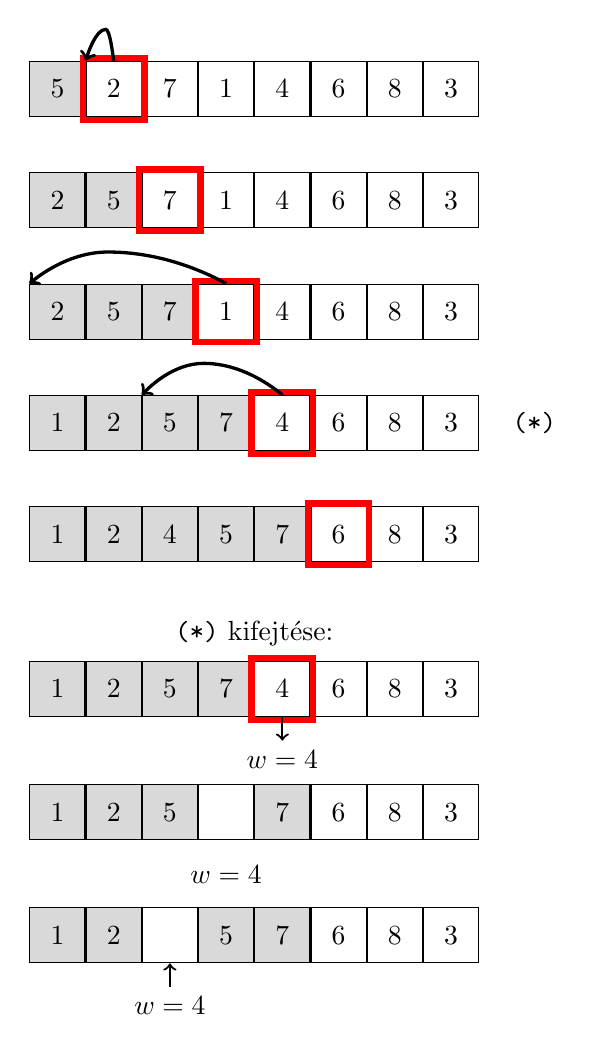
\begin{tikzpicture}
		\tikzmath{
			\nodeW       = 7;   %node width
			\nodeH       = 7;   %node height
			\figDist     = 7;   %distance between each fig
			\figDistW     = 8.5;  %distance between each fig after (*)
		}
		\tikzstyle{Base} = [
			text centered, 
			draw=black, 
			text centered,
			minimum width=\nodeW mm, 
			minimum height=\nodeH mm, 
		]
		\tikzstyle{LightNode} = [
			fill= white,
			Base
		]
		\tikzstyle{DarkNode} = [
			fill= gray!30,
			Base
		]
		\tikzstyle{Highlight} = [
			minimum width=\nodeW mm + 0.8mm, 
			minimum height=\nodeH mm+ 0.8mm, 
			draw = red,
			line width = 0.8mm
		]
		
		%%%%%%%%%%%%%%%%%%%%%%%%%%===---FIRST LINE---===%%%%%%%%%%%%%%%%%%%%%%%%%%
		\node (11) [DarkNode]{5};
			\node (12) [LightNode, right = 0mm of 11]{2};
			\node (13) [LightNode, right = 0mm of 12]{7};
			\node (14) [LightNode, right = 0mm of 13]{1};
			\node (15) [LightNode, right = 0mm of 14]{4};
			\node (16) [LightNode, right = 0mm of 15]{6};
			\node (17) [LightNode, right = 0mm of 16]{8};
			\node (18) [LightNode, right = 0mm of 17]{3};
		\node [Highlight] at ($(12)$) {};
		\draw [->, very thick] (12.north) parabola bend ($(12.north) + (-0.1,0.4)$) (11.north east);
		%%%%%%%%%%%%%%%%%%%%%%%%%%===---SECOND LINE---===%%%%%%%%%%%%%%%%%%%%%%%%%%
		\node (21) [DarkNode, below = \figDist mm of 11]{2};
			\node (22) [DarkNode, right = 0mm of 21]{5};
			\node (23) [LightNode, right = 0mm of 22]{7};
			\node (24) [LightNode, right = 0mm of 23]{1};
			\node (25) [LightNode, right = 0mm of 24]{4};
			\node (26) [LightNode, right = 0mm of 25]{6};
			\node (27) [LightNode, right = 0mm of 26]{8};
			\node (28) [LightNode, right = 0mm of 27]{3};
		\node [Highlight] at ($(23)$) {};
		%%%%%%%%%%%%%%%%%%%%%%%%%%===---THIRD LINE---===%%%%%%%%%%%%%%%%%%%%%%%%%%
		\node (31) [DarkNode, below = \figDist mm of 21]{2};
			\node (32) [DarkNode, right = 0mm of 31]{5};
			\node (33) [DarkNode, right = 0mm of 32]{7};
			\node (34) [LightNode, right = 0mm of 33]{1};
			\node (35) [LightNode, right = 0mm of 34]{4};
			\node (36) [LightNode, right = 0mm of 35]{6};
			\node (37) [LightNode, right = 0mm of 36]{8};
			\node (38) [LightNode, right = 0mm of 37]{3};
		\node [Highlight] at ($(34)$) {};
		\draw [->, very thick] (34.north) parabola bend ($(34.north) + (-1.5,0.4)$) (31.north west);
		%%%%%%%%%%%%%%%%%%%%%%%%%%===---FOURTH LINE---===%%%%%%%%%%%%%%%%%%%%%%%%%%
		\node (41) [DarkNode, below = \figDist mm of 31]{1};
			\node (42) [DarkNode, right = 0mm of 41]{2};
			\node (43) [DarkNode, right = 0mm of 42]{5};
			\node (44) [DarkNode, right = 0mm of 43]{7};
			\node (45) [LightNode, right = 0mm of 44]{4};
			\node (46) [LightNode, right = 0mm of 45]{6};
			\node (47) [LightNode, right = 0mm of 46]{8};
			\node (48) [LightNode, right = 0mm of 47]{3};
		\node [Highlight] at ($(45)$) {};
		\node [right = 3mm of 48]{\texttt{(*)}};
		%%%%%%%%%%%%%%%%%%%%%%%%%%===---FIFTH LINE---===%%%%%%%%%%%%%%%%%%%%%%%%%%
		\node (51) [DarkNode, below = \figDist mm of 41]{1};
			\node (52) [DarkNode, right = 0mm of 51]{2};
			\node (53) [DarkNode, right = 0mm of 52]{4};
			\node (54) [DarkNode, right = 0mm of 53]{5};
			\node (55) [DarkNode, right = 0mm of 54]{7};
			\node (56) [LightNode, right = 0mm of 55]{6};
			\node (57) [LightNode, right = 0mm of 56]{8};
			\node (58) [LightNode, right = 0mm of 57]{3};
		\node [Highlight] at ($(56)$) {};
		\draw [->, very thick] (45.north) parabola bend ($(45.north) + (-1,0.4)$) (43.north west);
		%%%%%%%%%%%%%%%%%%%%%%%%%%===---SEPARATOR LINE---===%%%%%%%%%%%%%%%%%%%%%%%%%%
		\node (dots) at ($(54.south east) + (0,-0.9)$) {\texttt{(*)} kifejtése:};
		%%%%%%%%%%%%%%%%%%%%%%%%%%===---SIXTH LINE---===%%%%%%%%%%%%%%%%%%%%%%%%%%
		\node (61) [DarkNode, below = \figDistW mm + 4mm of 51]{1}; %extra distance!
			\node (62) [DarkNode, right = 0mm of 61]{2};
			\node (63) [DarkNode, right = 0mm of 62]{5};
			\node (64) [DarkNode, right = 0mm of 63]{7};
			\node (65) [LightNode, right = 0mm of 64]{4};
			\node (66) [LightNode, right = 0mm of 65]{6};
			\node (67) [LightNode, right = 0mm of 66]{8};
			\node (68) [LightNode, right = 0mm of 67]{3};
		\node [Highlight] at ($(65)$) {};
		\node (w1) [below = 3 mm of 65] {$w=4$};
		\draw [->, thick] (65) -- (w1);
		%%%%%%%%%%%%%%%%%%%%%%%%%%===---SEVENTH LINE---===%%%%%%%%%%%%%%%%%%%%%%%%%%
		\node (71) [DarkNode, below = \figDistW mm of 61]{1};
			\node (72) [DarkNode, right = 0mm of 71]{2};
			\node (73) [DarkNode, right = 0mm of 72]{5};
			\node (74) [LightNode, right = 0mm of 73]{};
			\node (75) [DarkNode, right = 0mm of 74]{7};
			\node (76) [LightNode, right = 0mm of 75]{6};
			\node (77) [LightNode, right = 0mm of 76]{8};
			\node (78) [LightNode, right = 0mm of 77]{3};
		\node (w2) [below = 2 mm of 74] {$w=4$};
		%%%%%%%%%%%%%%%%%%%%%%%%%%===---EIGHTH LINE---===%%%%%%%%%%%%%%%%%%%%%%%%%%
		\node (81) [DarkNode, below = \figDistW mm of 71]{1};
			\node (82) [DarkNode, right = 0mm of 81]{2};
			\node (83) [LightNode, right = 0mm of 82]{};
			\node (84) [DarkNode, right = 0mm of 83]{5};
			\node (85) [DarkNode, right = 0mm of 84]{7};
			\node (86) [LightNode, right = 0mm of 85]{6};
			\node (87) [LightNode, right = 0mm of 86]{8};
			\node (88) [LightNode, right = 0mm of 87]{3};
		\node (w3) [below = 3 mm of 83] {$w=4$};
		\draw [->, thick] (w3) -- (83);
		
	\end{tikzpicture}
\end{document}